\chapter{Introduction}

\section{Kubernetes}

In this section we will dive into the topic of Kubernetes. We start by shortly overviewing the Kubernetes architecure. Then we expand on the Kubernetes resources, their kinds and their role in the target application environment. Finally, we consider the security of Kubernetes.

\subsection{Overview}

Kubernetes, also known as K8s, is an open source system for automating deployment, scaling, and management of containerized applications. It groups containers that make up an application into logical units for easy management and discovery. Kubernetes builds upon 15 years of experience of running production workloads at Google, combined with best-of-breed ideas and practices from the community. \cite{kubernetes}.

IBM defines Kubernetes as an open source \textbf{container orchestration platform} for scheduling and automating the deployment, management and scaling of containerized applications. Today, Kubernetes and the broader ecosystem of container-related technologies have merged to form the building blocks of modern cloud infrastructure. This ecosystem enables organizations to deliver a highly productive hybrid multicloud computing environment to perform complex tasks surrounding infrastructure and operations. It also supports cloud-native development by enabling a build-once-and-deploy-anywhere approach to building applications. \cite{ibm-kubernetes}.

It is important to emphasize that the Kubernetes abstracts the actual machines (nodes) from the user. Nodes can be physical on-premises servers, or VMs that reside either on-premises or at a cloud provider. Kubernetes takes on the responsibilty of figuring out the deployment target for a particular application. That is, user only defines the desired state of the infrastructure using YAML or JSON configuration files. Kubernetes then creates all the workloads based on the applied configuration.

\subsection{Kubernetes Architecture}

While Kubernetes requires at least three nodes to run, there are some implementation designed for the local use, which emulate this concept (see Subsection~\ref{sec:other-kubernetes-implementations}). The master node is called control plane. The control plane manages the worker nodes and the Pods in the cluster. In production environments, the control plane usually runs across multiple computers and a cluster usually runs multiple nodes, providing fault-tolerance and high availability. Worker nodes host the actual workload inside the cluster. Figure~\ref{img:kubernetes-architecture} provides a simple high-level overview of a typical Kubernetes cluster with a Control Plane and three worker nodes.

\begin{figure}[!hbt]
	\begin{center}
		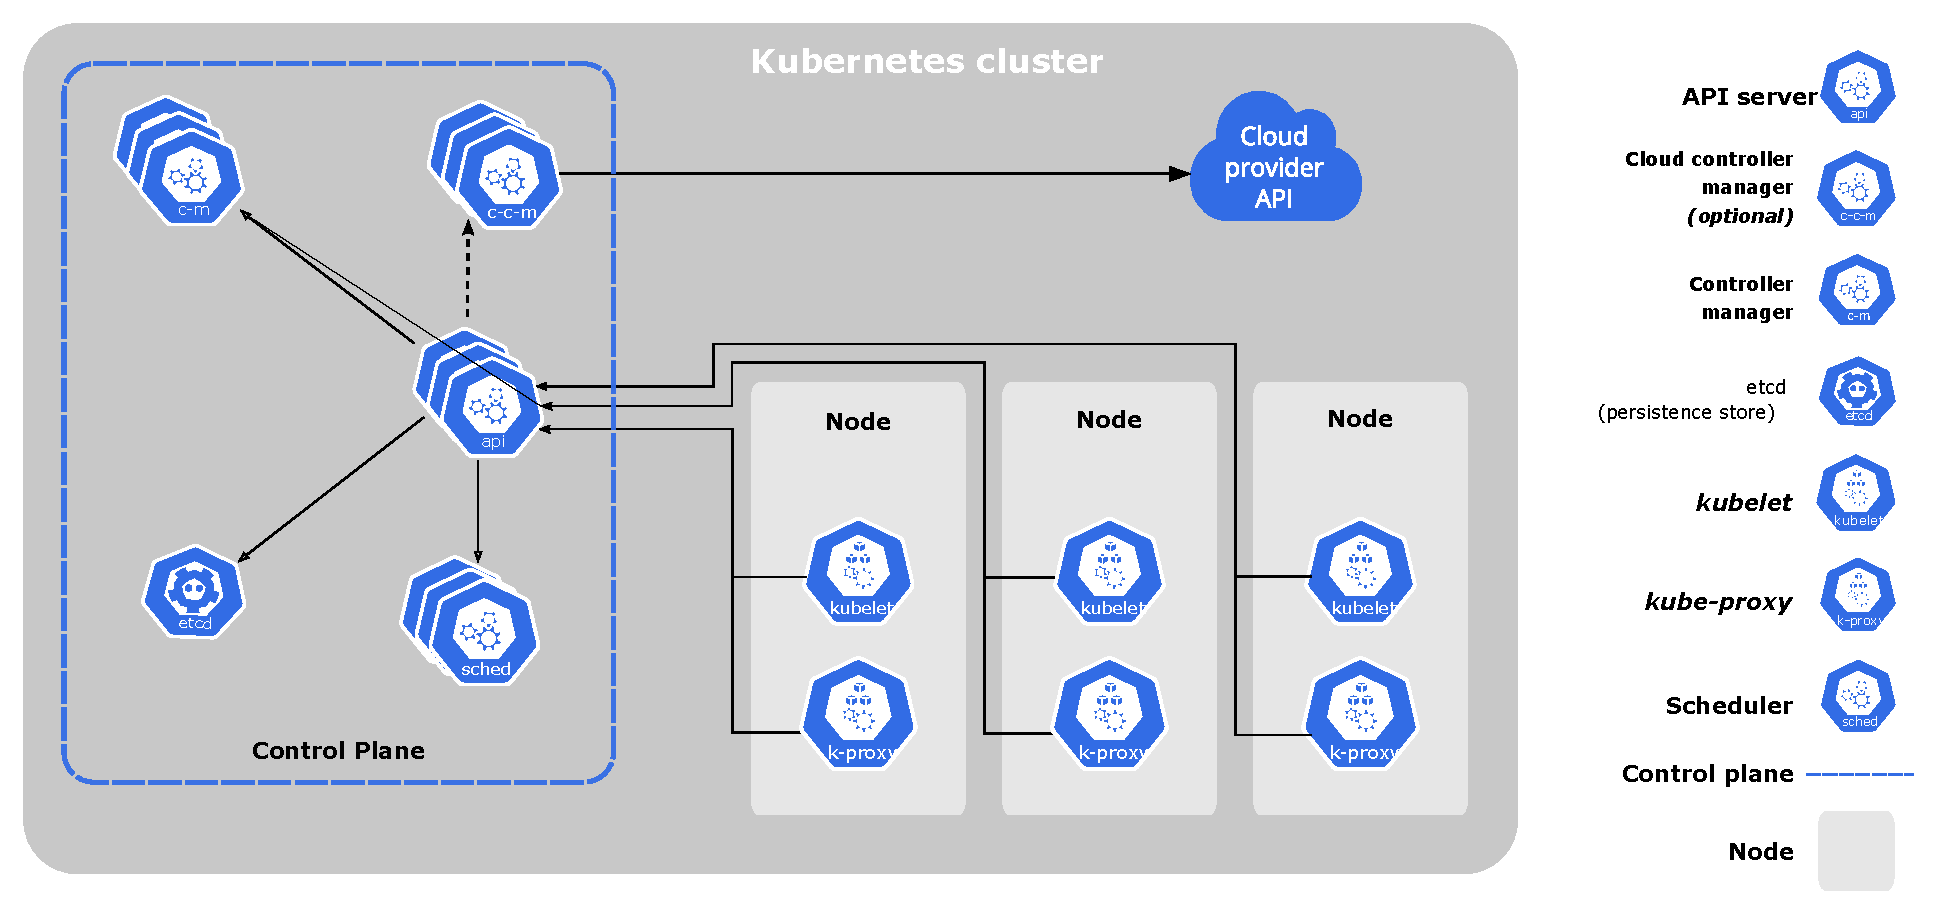
\includegraphics[width=0.85\textwidth]{images/components-of-kubernetes.pdf}
        \caption{Kubernetes cluster architecure overview with its main components.}
		\label{img:kubernetes-architecture}
	\end{center}
\end{figure}

\subsubsection*{Control Plane overview}

Control plane runs the following components: 
\begin{itemize}
\item \textbf{kube-apiserver} \\
Kube-apiserver exposes the Kubernetes API, which is acting as a frontend for the Kubernetes control plane.
\item \textbf{etcd} \\
Etcd is a key-value store, where all of the cluster data is stored.
\item \textbf{kube-scheduler} \\
Each time a new pod is created, it is passed to the kube-scheduler, which assigns the pod to the specific node to run on (based on individual and collective resource requirements, hardware/software/policy constraints, affinity and anti-affinity specifications, data locality, inter-workload interference, and deadlines).
\item \textbf{kube-controller-manager} \\
Each Kubernetes resource has its own controller (e.g. NodeController, JobController, ServiceAccountController); all of them are compiled as one binary called kube-controller-manager.
\item \textbf{cloud-controller-manager} \\
Cloud-controller-manager embeds cloud-specific control logic. It differs depending on the cloud provider or can be absent completely, when running Kubernetes locally.
\end{itemize}

\subsubsection*{Worker Node overview}

Each worker node has a kubelet and kube-proxy installed. Kubelet is an agent that manages runnning pods and containers. Kube-proxy is a network proxy that implements parts of the Kubernetes service concept. It maintains network rules on nodes, making in- outside-cluster communitcation possible.

Then, of course, each worker node has a set of running pods. A typical use would involve multiple running applications. Depending on the size of the node and the application resoucre consumption it can accomodate on average from one to a few dozens applications with various business purposes.

\subsection{Kubernetes Resources}

Kubernetes resources are fundamental components that define various entities within a Kubernetes cluster. Resources are objects that represent the desired state and configuration of the infrastructure, applications, and services running on the cluster. Kubernetes provides a range of resources that enable developers and operators to define, manage, and scale containerized applications, network policies, storage requirements, and more. These resources are defined declaratively in YAML or JSON files, which makes infrastructure setup consistent and reproducible.

Among key Kubernetes resoucres are:
\begin{itemize}
    \item \textbf{Pods} \\
        Pod is the atomic workload unit in the Kubernetes cluster. It encapsulates one or more containers that share the same network. It represents a single instance of a running application.
    \item \textbf{Deployments} \\
        Deployments are a higher level of abstraction for the Pods. They allow to define replica count and rollout/rollback strategy for the updates, which can be used to ensure availability for the application.
    \item \textbf{Services} \\
        Services provide a communication layer for the pods inside one cluster. Being an abstraction over the pods' network, they provide reliable access to the selected workloads, while serving as a Load Balancer. 
    \item \textbf{ConfigMaps} and \textbf{Secrets} \\
        ConfigMaps and Secrets allow users to store data outside the workload. ConfigMaps are usually used to store non-sensitive information like environment and application configuration parameters. Secrets are a more secure resource designed for API keys, passwords and other sensitive data.
    \item \textbf{PersistentVolumes} and \textbf{PersistentVolumeClaims} \\
        These resources enable stateful applications to request and mount durable storage within a cluster, allowing data to persist independently of the Pod lifecycle.
\end{itemize}

Above are the most commonly used resources, which we also leverage in the practical part of the paper. Therefore, it is important that the reader understands the position and the purpose of each resource in the cluster infrastructure.

\subsubsection*{Workloads}

Minimal computing units in Kubernetes are Containers, which are running in Pods. However, to simplify the management of Pods, Kubernetes has workload resources, which manage the set of Pods. They make sure the desired number of Pods of right kind are running to match the declaration.

Deployments and ReplicaSets are a good fit for stateless applications. Each pod in the Deployment is interchangebeable. Deployments are easily scalable and have built-in versioning and rollout mechanisms.

StatefulSet allows to create sets of stateful applications. They might share the same PersistentVolume and replicate data between each other.

DaemonSet defines Pods that provide node-local facilities. These might be fundamental to the operation of your cluster, such as a networking helper tool, or be part of an add-on.

Job and CronJob define tasks that run to completion and then stop. Jobs represent one-off tasks, whereas CronJobs recur according to a schedule.

\subsubsection*{Networking}

Kubernetes networking model makes Pods look like VMs in the networking aspect. Pods on any nodes can communicate with each other without NAT. Containers inside the same Pod share its network meaning that they can reach each other using localhost.

Kubernetes networking addresses four concerns:
\begin{itemize}
\item Containers within a Pod use networking to communicate via loopback.
\item Cluster networking provides communication between different Pods.
\item The Service API lets you expose an application running in Pods to be reachable from outside your cluster.
\item Ingress provides extra functionality specifically for exposing HTTP applications, websites and APIs.
\item You can also use Services to publish services only for consumption inside your cluster.
\end{itemize}

\subsubsection*{Storage}

Kubernetes does not ship a particular implementation of storage. However, it provides a range of resources that define the storage concept and supports different types of volumes. A Pod can use any number of volume types simultaneously. Ephemeral volume types have a lifetime of a pod, but persistent volumes exist beyond the lifetime of a pod. When a pod ceases to exist, Kubernetes destroys ephemeral volumes; however, Kubernetes does not destroy persistent volumes. For any kind of volume in a given pod, data is preserved across container restarts.

At its core, a volume is a directory, possibly with some data in it, which is accessible to the containers in a pod. How that directory comes to be, the medium that backs it, and the contents of it are determined by the particular volume type used.

PersistentVolumes and PersistentVolumeClaims are the resources kinds most important to understand here.
\begin{itemize}
\item A PersistentVolume (PV) is a piece of storage in the cluster that has been provisioned by an administrator or dynamically provisioned using Storage Classes. It is a resource in the cluster just like a node is a cluster resource. PVs are volume plugins like Volumes, but have a lifecycle independent of any individual Pod that uses the PV. This API object captures the details of the implementation of the storage, be that NFS, iSCSI, or a cloud-provider-specific storage system.
\item A PersistentVolumeClaim (PVC) is a request for storage by a user. It is similar to a Pod. Pods consume node resources and PVCs consume PV resources. Pods can request specific levels of resources (CPU and Memory). Claims can request specific size and access modes (e.g., they can be mounted ReadWriteOnce, ReadOnlyMany or ReadWriteMany). Once and Many here refer to a number of Pods that can perform the read or write simultaneously.
\end{itemize}

\subsection{Infrastructure Security}

When we are talking about the infrastructure security, we must consider multiple layers. Going from the top to the bottom, we start with the security measurements taken on the Cloud provider side. In most cases this is not something we can affect and the security of different Cloud providers varies significantly. Unfortunately, this is out of scope of this paper, but all of the "big five" Cloud providers (AWS, Azure, Google Cloud, Alibaba and IBM) maintain high security standarts and security risks generally should not be a concern for their end users. Then, we get to the cluster itself. On the cluster level we must consider the security of the nodes, security of the cluster components and their configuration. At this layer we have already some space for the misconfigurations to appear. Here we can evaluate the security of the single components using some of the security scanners presented in \nameref{sec:kubernetes-security-automation}. Lastly, we get to the application level, where the security of the application code, Kubernetes resoucre configuration, libraries, dependencies and base images is the main concern. Again, this is the layer, where the developers have the most access to, thus, providing a lot of space for the possibility of a human error. In this paper we mostly work on this level when we do our research.

Officially, The Linux Foundation provides only some security guidelines for each of the layers. However, bundled with Kubernetes we get a few means to keep the security under control. Below we present an overview of the Kubernetes security recommendations, RBAC and Data security inside Kubernetes.

\subsubsection*{Kubernetes security recommendations}

This section gathers the official security recommendations provided by the Kubernetes. They provide a list of concerns for each level of the cloud infrastructure. Cloud infrastructure can be viewed as a composition of four layers as displayed by the Figure~\ref{img:cloud-security}.

\begin{figure}[!hbt]
	\begin{center}
		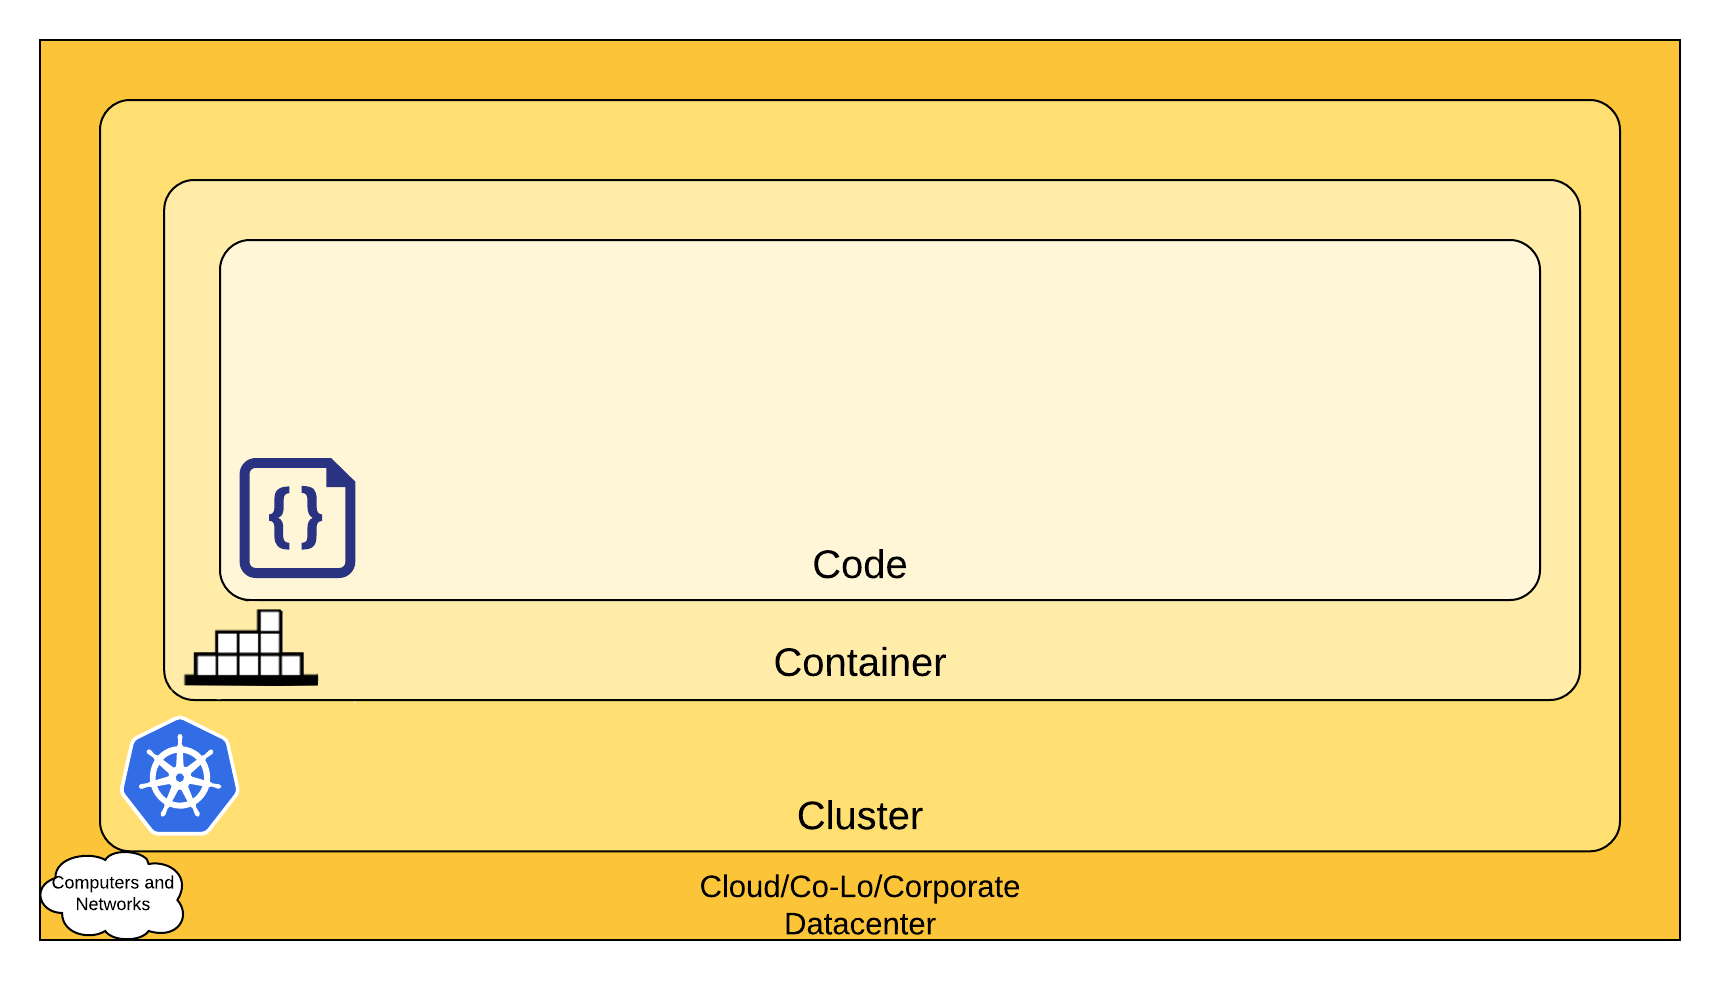
\includegraphics[width=0.75\textwidth]{images/cloud-security.png}
        \caption{Four layers of the cloud infrastructure.}
		\label{img:cloud-security}
	\end{center}
\end{figure}

Each layer is built upon the previous one and its security depends on the security of the outer layers. It is, therefore, important to maintain high security standarts on base levels (Cloud, Cluster, Container).

\begin{enumerate}

\item \textbf{Cloud} \\
Each cloud provider has its own security policies and guidelines. There are, however, some general infrastructure-level security best advice described by in the Table~\ref{tab:cloud-security-recommendations}.

\begin{table}[H]
    \begin{center}
        \begin{tabular}{ | p{.20\textwidth} | p{.80\textwidth} | } 
         \hline
         \textbf{Area of Concern for Kubernetes Infrastructure} & \textbf{Recommendation} \\ 
         \hline
         Network access to API Server (Control plane) & All access to the Kubernetes control plane is not allowed publicly on the internet and is controlled by network access control lists restricted to the set of IP addresses needed to administer the cluster. \\ 
         \hline
         Network access to Nodes (nodes)  & Nodes should be configured to only accept connections (via network access control lists) from the control plane on the specified ports, and accept connections for services in Kubernetes of type NodePort and LoadBalancer. If possible, these nodes should not be exposed on the public internet entirely. \\ 
         \hline
         Kubernetes access to Cloud Provider API & Each cloud provider needs to grant a different set of permissions to the Kubernetes control plane and nodes. It is best to provide the cluster with cloud provider access that follows the principle of least privilege for the resources it needs to administer. \\
         \hline
         Access to etcd & Access to etcd (the datastore of Kubernetes) should be limited to the control plane only. Depending on your configuration, you should attempt to use etcd over TLS. \\
         \hline
         etcd Encryption & Wherever possible it's a good practice to encrypt all storage at rest, and since etcd holds the state of the entire cluster (including Secrets) its disk should especially be encrypted at rest. \\
         \hline
        \end{tabular}
    \end{center}
    \caption{Security recommendations for the Cloud layer.}
    \label{tab:cloud-security-recommendations}
\end{table}

\item \textbf{Cluster} \\
There are two cluster security concerns that could be addressed: securing the configurable cluster components and securing the applications running in the cluster.

There are a few things to consider regarding the application security:
\begin{itemize}
\item RBAC Authorization (Access to the Kubernetes API)
\item Authentication	
\item Application secrets management (and encrypting them in etcd at rest)
\item Ensuring that pods meet defined Pod Security Standards
\item Quality of Service (and Cluster resource management)
\item Network Policies
\item TLS for Kubernetes Ingress
\end{itemize}

\item \textbf{Container} \\
Securing containers is a vast topic, which deserves its own chapter. There are, nevertheless, a few general recommendation provided by the Kubernetes, which you can find in the Table~\ref{tab:container-security-recommendations}.

\begin{table}[H]
    \begin{center}
        \begin{tabular}{ | p{.20\textwidth} | p{.80\textwidth} | } 
        \hline
        \textbf{Area of Concern for Containers} & \textbf{Recommendation} \\ 
        \hline
        Container Vulnerability Scanning and OS Dependency Security & As part of an image build step, you should scan your containers for known vulnerabilities. \\ 
        \hline
        Image Signing and Enforcement & Sign container images to maintain a system of trust for the content of your containers. \\ 
        \hline
        Disallow privileged users & When constructing containers, create users inside of the containers that have the least level of operating system privilege necessary in order to carry out the goal of the container. \\
        \hline
        \end{tabular}
    \end{center}
    \caption{Security recommendations for the Container layer.}
    \label{tab:container-security-recommendations}
\end{table}

\item \textbf{Code} \\
When it comes to code, the developers have the most flexibility to design secure applications. There are a lot of issues to address, which may vary significantly from application to application depending on its purpose, architecture and framework base. Kubernetes documentation gives a handful of recommendations regarding this topic, which are displayed below in the Table~\ref{tab:code-security-recommendations}.

\begin{table}[H]
    \begin{center}
        \begin{tabular}{ | p{.20\textwidth} | p{.80\textwidth} | } 
        \hline
        \textbf{Area of Concern for Code} & \textbf{Recommendation} \\ 
        \hline
        Access over TLS only & If your code needs to communicate by TCP, perform a TLS handshake with the client ahead of time. With the exception of a few cases, encrypt everything in transit. Going one step further, it's a good idea to encrypt network traffic between services. This can be done through a process known as mutual TLS authentication or mTLS which performs a two sided verification of communication between two certificate holding services. \\ 
        \hline
        Limiting port ranges of communication & This recommendation may be a bit self-explanatory, but wherever possible you should only expose the ports on your service that are absolutely essential for communication or metric gathering. \\ 
        \hline
        3rd Party Dependency Security & It is a good practice to regularly scan your application's third party libraries for known security vulnerabilities. Each programming language has a tool for performing this check automatically. \\
        \hline
        Static Code Analysis & Most languages provide a way for a snippet of code to be analyzed for any potentially unsafe coding practices. Whenever possible you should perform checks using automated tooling that can scan codebases for common security errors. \\
        \hline
        Dynamic probing attacks & There are a few automated tools that you can run against your service to try some of the well known service attacks. These include SQL injection, CSRF, and XSS. One of the most popular dynamic analysis tools is the OWASP Zed Attack proxy tool. \\
        \hline
        \end{tabular}
    \end{center}
    \caption{Security recommendations for the Code layer.}
    \label{tab:code-security-recommendations}
\end{table}
                      
\end{enumerate}

\subsubsection*{Role Based Access Control}

\subsubsection*{Data security}

\subsection{Other Kubernetes Implementations}
\label{sec:other-kubernetes-implementations}

\subsubsection*{Openshift}

\subsubsection*{Rancher Desktop}
\section{Kubernetes security automation}
\label{sec:kubernetes-security-automation}

This section introduces the reader to the topic of the security automation inside the Kubernetes cluster. We discuss different security tools, their place in the cloud Infrastructure and examine their usage patterns. Additionally, we explain why were the specific tools chosen for our research.

\subsection{Overview}

Kubernetes security scanners and operators provide an array of defensive capabilties. Most of them act in the form of informator. That is, they do not perform any remediatory actions, but only provide user with information about the cluster security status. Nevertheless, there are some solutions on the market that are capable of resolving some of the security issues automatically. This, on the other hand, introduces another layer of concern: can we really trust a third-party system to introduce modifications to our infrastructure? That the former type is the most abundant and is the focus of this paper. Automatic remediation can be then implemented as a part of CI/CD pipeline based on the scan results. This ensures that it is compliant with the company's policies and is tailored to the company's needs.

One of the ways to classify Kubernetes security scanners is by the scan target. Here we can roughly divide them into three groups: configuration file scanners, cluster scanners and container image scanners. Most of the tools, however, can be put into multiple different groups. Cluster scanners usually are able to perform container image scanning as well and it is a part of the full cluster scan. Cluster scanners detect misconfigurations in the cluster infrastructure and its essential components. They look for, among other things, containers running with extensive privilages, exposed sensitive workloads and plaintext secrets. Container image scanners look for known vulnerabilities inside the images. Configuration file scanners perform a scan of the cluster configuration files. For large infrastructure with a number of applications deployed there might be over several tens of thousands lines of configuration and such scanners aim to detect any known misconfigurations by going through theese lines.

Cluster security scanners can be further classified by the execution point. Again, there is usually more than one way to run a scan, but here are a few options: run a scanner tool as a container, run it from a remote machine connected to the cluster, run it is an operator, which can perform scan automatically on a regular basis. To always keep cluster up-to-date with the most recent security patches the best solution would be to either install an operator or integrate a security scanner tool into your CI/CD pipeline.

\subsection{Selection Criteria}

To perform our assessment we have chosen from a variety of Kubernetes security scanners. Though the area is still relatively new, there is a variety of tools with different purposes available on the market. We made our choice based on the following criteria:
\begin{itemize}
\item \textbf{free-to-use} \\
We do include some proprietary tool testing further in our research as an additional comparison, however, for the main part we only use free tools. Kubernetes itself is distributed under Apache License 2.0, which means it is inherently free to use. The ability to adopt these tools without financial constraints enables wider adoption, thus, contributing to the community-driven innovations. Finally, this research not being funded, we could only afford to work with openly distributed software.
\item \textbf{open-source} \\
Again, we are sticking to the open-source nature of the Kubernetes. By selecting open-source tools, this research ensures that each tool's codebase is transparent and can be reviewed by security experts. This transparency increases trust in the tools' effectiveness, as the community can spot, disclose, and even patch any vulnerabilities in the software. Another advantage is the customization of the open-source software as the companies can adapt the tools to their specific Kubernetes security needs.
\item \textbf{designed with cloud in mind} \\
Designed to be used in the Kubernetes environment specifically, these tools should offer features like scanning container images for vulnerabilities, but also monitoring network policies, securing Kubernetes configuration files, or identifying misconfigurations within clusters. Tools built specifically for Kubernetes are more efficient, as they are optimized to address the distinct aspects of the platform, making security management more effective.
\item \textbf{has an active community support} \\
Tools with active communities tend to have more frequent updates, faster response times for bug fixes, and a wide range of contributors who bring diverse insights to improve functionality and security. The world of the software security is changing rapidly and an active community means that the tool is up-to-date with the most recent events. A thriving community also means that users can easily access support on the community forums.
\end{itemize}

Based on the aforementioned criteria we ended up choosing and testing the following tools:
\begin{itemize}[noitemsep]
\item Trivy
\item Kube-bench
\item Prowler
\item Kubescape
\end{itemize}

In the next chapters we closely examine each selected tool and explain how it is matches our selection criteria. Additionally, we compare them to each other and highlight their strong and weak sides.

\subsection{Trivy}
Trivy is an Aqua Security open source project with a vast array of use cases. It supports multiple scan targets and includes multiple scanners. Among the supported targets are:
\begin{itemize}[noitemsep]
    \item Container Image
    \item Filesystem
    \item Git Repository 
    \item Virtual Machine Image
    \item Kubernetes
\end{itemize}
Trivy includes scanners for:
\begin{itemize}[noitemsep]
    \item OS packages and software dependencies in use (SBOM)
    \item Known vulnerabilities (CVEs)
    \item IaC issues and misconfigurations
    \item Sensitive information and secrets
    \item Software licenses
\end{itemize}

According to the Trivy official Gihub page \cite{trivy-github}, it can be installed on the local machine using any of the popular package mangager or by downloading a binary from the Github Releases. It can also be ran as a Docker container or Kubernetes Operator. Furthermore, Trivy can be integrated into GitHub Actions or installed as a Visual Studio Code plugin. Aqua Security uploads each new release as a Docker image into the Dockerhub repository. There is a variety of supported configuration parameters for Trivy Kubernetes scanning feature. Users can specify which scanners to include, which namespaces to skip, which nodes to scan and the format of the output. An example of a Trivy misconfiguration scan command executed against the default Kubernetes context, which would output a short summary of findings and skip \textbf{dev-system} namespace, is included below (see Listing~\ref{lst:trivy-k8s}).

\begin{center}
    \begin{lstlisting}[language=bash, caption={[An example of a Trivy Kubernetes scan command] An example of a Trivy Kubernetes scan command.}, label={lst:trivy-k8s}]
    $ trivy k8s \
        --scanners=misconfig \
        --report=summary \
        --exclude-namespace=dev-system
    \end{lstlisting}
\end{center}

Since Kubernetes is listed as a natively supported target and Trivy can scan for both vulnerabilities and misconfigurations, Trivy is well-suited for our research. It is also open source and available for free. Presently, Trivy's Github repository has over 2800 issues, with a little over than 150 of them being open, repository's commit history shows active development with a bi-monthly minor release cycle and yearly major release cycle. Thus, we can assume an active community and developer support.

\subsection{Kube-bench}
Kube-bench is another open source tool developed by Aqua Security. Their Github page \cite{kube-bench-github} states that it checks whether Kubernetes is deployed securely by running the checks against the CIS Kubernetes Benchmark (see \ref{sss:cis-kubernetes-benchmark}). Kube-bench is designed specifically for Kubernetes. Users can run the it inside a Docker container or deploy it as a Kubernetes job, however, there is still an option to download the binary on the local machine and run it against the desired Kubernetes cluster.

Since kube-bench has a much narrower feature set than Trivy, it is much more simple in usage, but still highly configurable. Configuration can be supplied via a config file or we can pass the configuration parameters directly using one of the 24 flags. An example of a simple scan command targeting \textbf{master}, \textbf{node}, \textbf{etcd}, \textbf{policies} CIS Benchmark categories is provided in Listing~\ref{lst:kube-bench-scan}.

\begin{center}
    \begin{lstlisting}[language=bash, caption={[An example of a Kube-bench scan command] An example of a Kube-bench scan command.}, label={lst:kube-bench-scan}]
    $ kube-bench run \
        --targets master,node,etcd,policies
    \end{lstlisting}
\end{center}

Kube-bench is actively supported by the developers and the community. At the present moment, Kube-bench Github repository has about 500 issues, 10\% of which are currently open. Repository receives updates on a weekly basis and the new version is released monthly.

\subsection{Prowler}

Prowler, as described on the Github page \cite{prowler-github}, is an open source security tool designed to perform Kubernetes security best practices assessments, audits, incident response, continuous monitoring, hardening and forensics readiness, and remediation. It is shipped with a built-in dashboard, which displays scan results in graphical format (see Fig~\ref{img:prowler-dashboard}). However, the dashboard can only read the scan results from the folder on the host machine and the user cannot trigger a new scan directly from the dashboard. Users have to install a separate Prowler App inside the clusters to trigger the scan. According to the documentation \cite{prowler-app-page}, ``it provides a user-friendly interface to configure and run scans, view results, and manage your security findings.''

\begin{figure}[!hbt]
	\begin{center}
		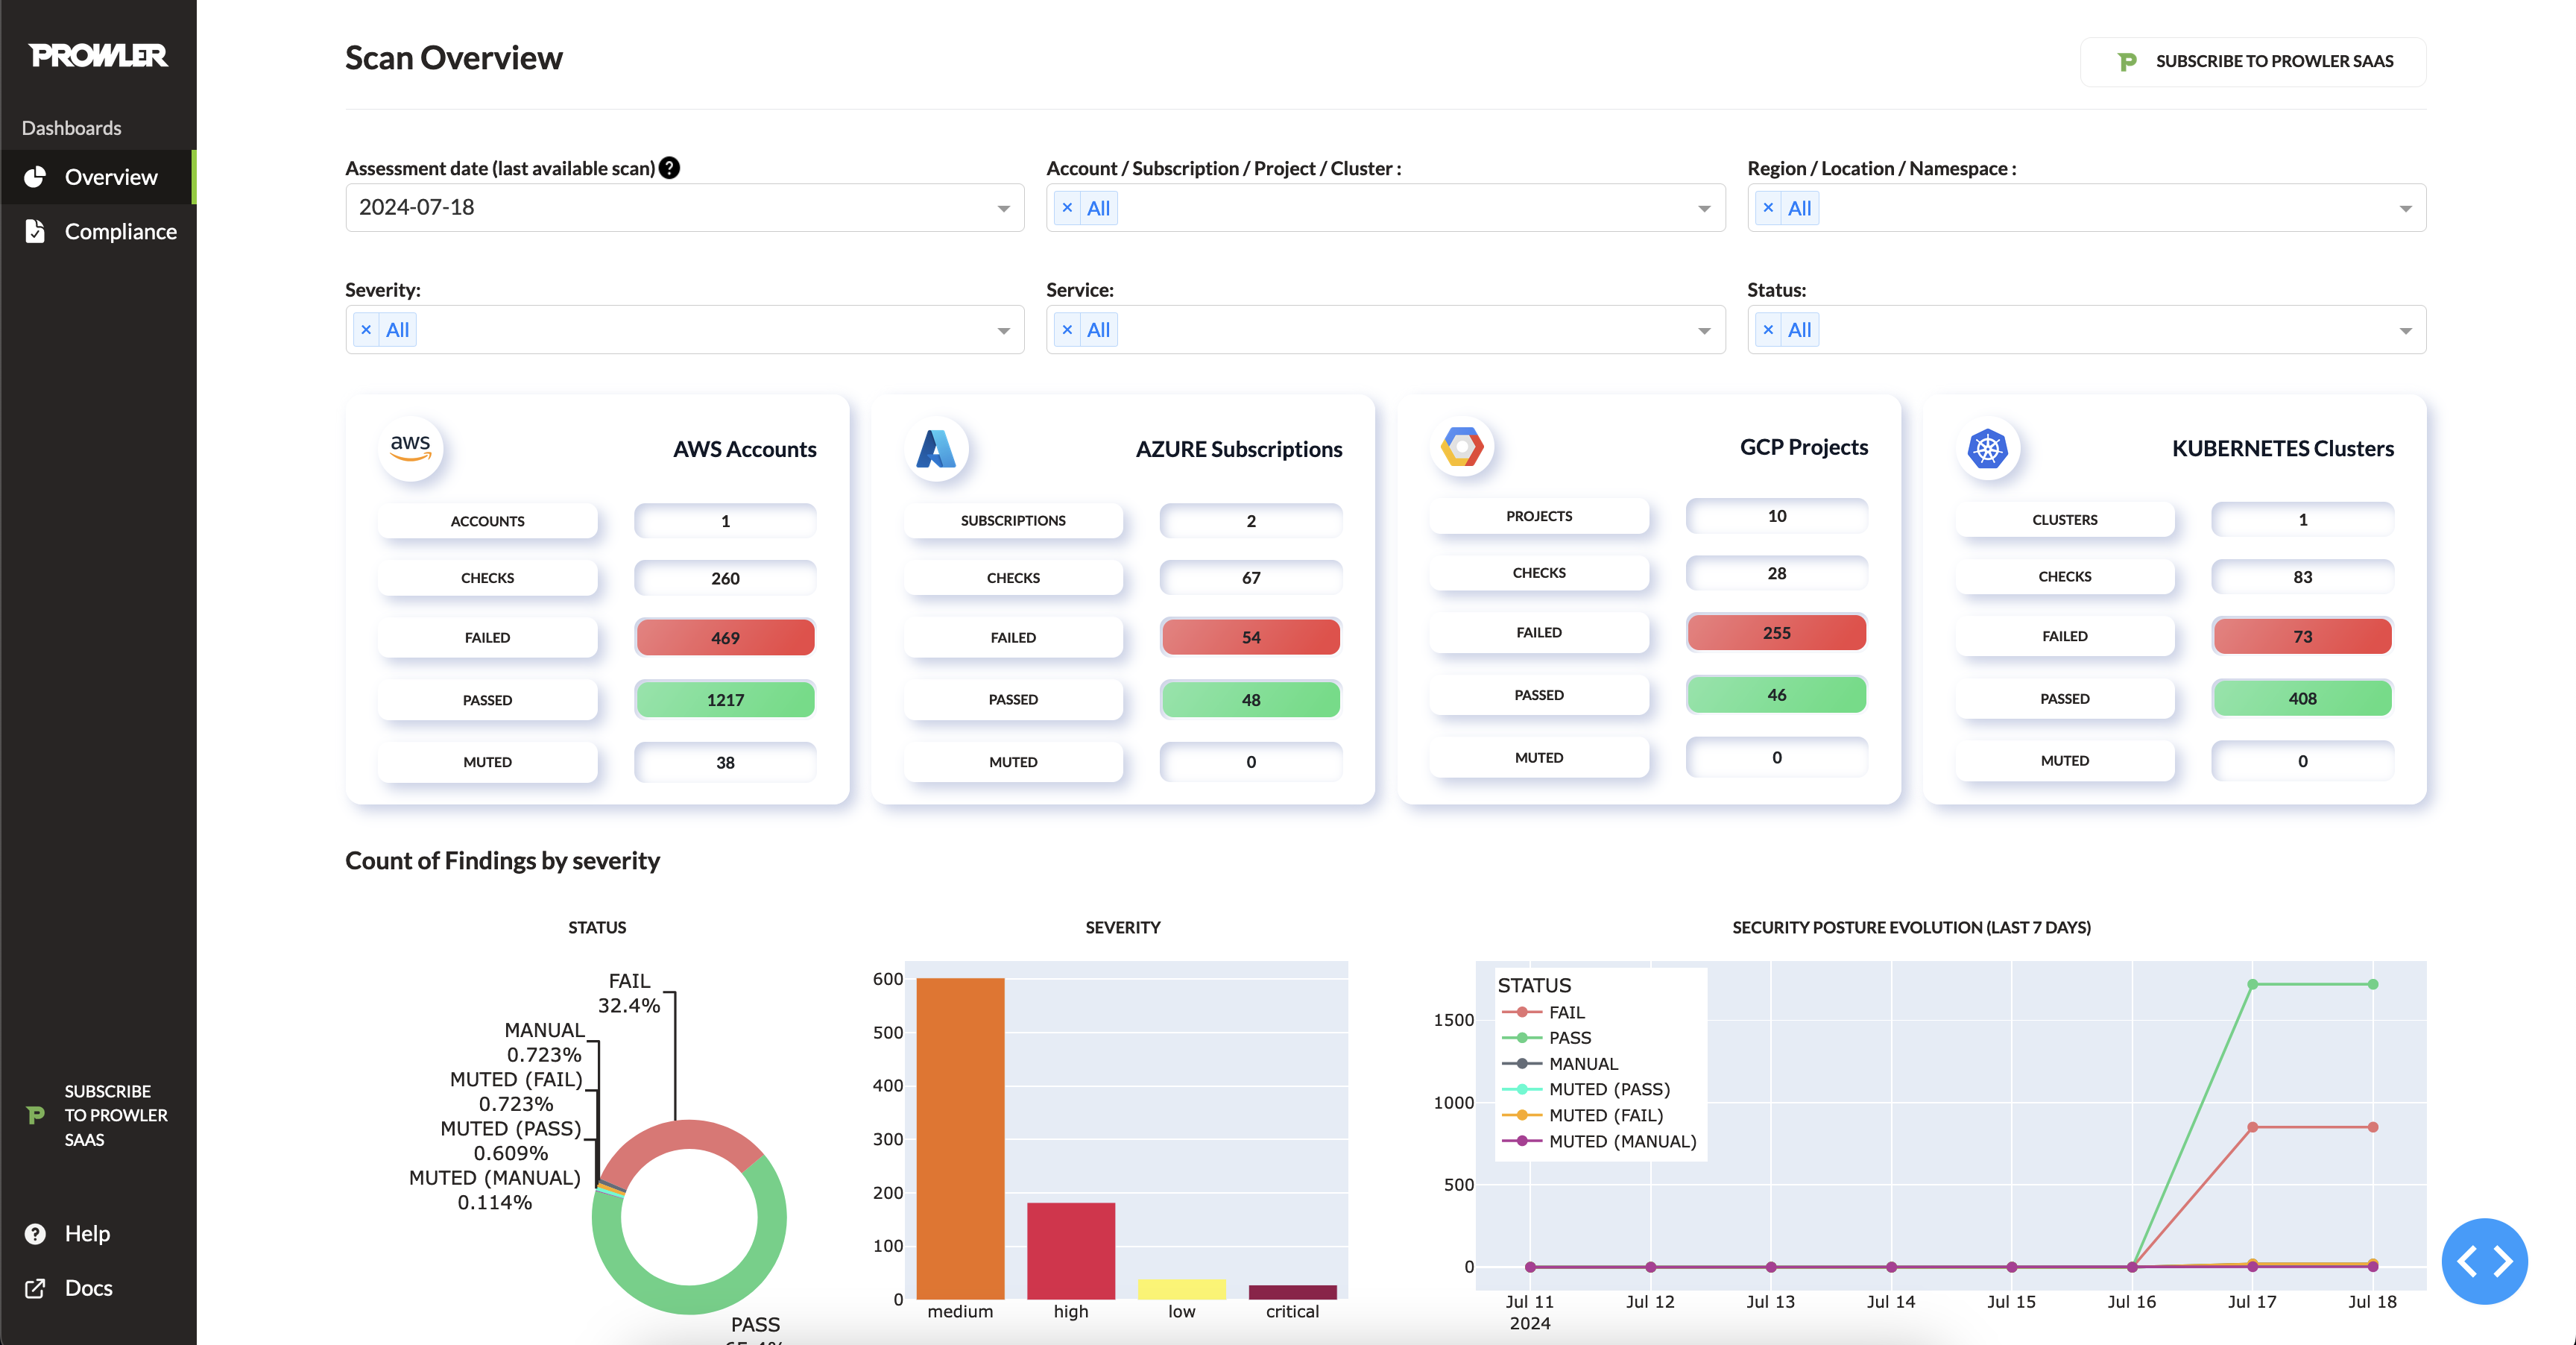
\includegraphics[width=0.85\textwidth]{images/prowler-dashboard.png}
        \caption{Prowler dashboard interface.}
		\label{img:prowler-dashboard}
	\end{center}
\end{figure}

Prowler CLI supports Azure, Google Cloud, AWS and generic Kubernetes providers. It performs a scan against multiple Kubernetes security frameworks to ensure the best coverage. Prowler supports output in CSV or JSON-OCSF format, the latter being an independent open source developed JSON schema by Open Cybersecurity Schema Framework project, which has recently joined the Linux Foundation organization. Again, we configure the Prowler job either via a configuration file or by passing the flags directly in the execution command. Listing~\ref{lst:prowler-command} provides an example on how can a Prowler scan be triggered. This particular execution would output the results in \textbf{json-ocsf} format, including only failed and manual checks.

\begin{center}
    \begin{lstlisting}[language=bash, caption={[An example of a Prowler scan command] An example of a Prowler scan command.}, label={lst:prowler-command}]
    $ prowler kubernetes \ 
        --status FAIL,MANUAL \
        --output-formats json-ocsf
    \end{lstlisting}
\end{center}

There are over a thousand issues in official Prowler Github repository. The development is still in progress and the tool receives regular updates. The project has an active community with operational development support.

\subsection{Kubescape}
Kubescape is an open-source security platform designed to harden the security of a Kubernetes cluster. Kubescape CLI allows users to scan the cluster from the local machine. Kubescape Operator enables image vulnerability scanning as well as continuous and scheduled scanning. Kubescape also offers Github Actions integration for CI/CD pipelines according to the official Github page \cite{kubescape-github}.

Kubernetes cluster is verified against a posture library (available at Github \cite{regolibrary-github}), which is a collection of frameworks each containing a set of controls. By default, the library is comprised of NSA Framework controls, MITRE ATT\&CK Framework controls and CIS Benchmark controls.

Scan configuration is again passed with multiple flags. There are flags allowing to select the namespaces to include into scan, namespaces to exclude from the scan, output format and location. Scanning can be then performed using the command displayed in Listing~\ref{lst:kubescape-command}.

\begin{lstlisting}[language=bash, caption={[An example of a Kube-bench scan command] An example of a Kube-bench scan command.}, label={lst:kubescape-command}]
    $ kubescape scan \
        --format json \
        --output kubescape-scan.json
\end{lstlisting}

Unfortunately, when executed in this mode, Kubescape performs only a few checks. In order to perform complete vulnerability and misconfiguration scan, Kubescape requires Kubescape Operator installed in the cluster. 

Kubescape's repository shows ongoing development with regular update releases.

\subsection{Preliminary Comparison}

This section compares the selected tools based on their declared feature set, ease of installation and execution, scan targets, supported cloud providers and security frameworks. This comparison does not include the analysis of the scan results, performance or any other aspects of execution. A detailed analysis of the generated reports can be found in Chapter~\ref{chap:results}.

We start by comparing the scanners by their feature set. Trivy has the most broad feature set as it is able to scan for vulnerabilities inside the images, perform IaC scan (supporting Terraform, Helm, plain Kubernetes YAML), scan for misconfigurations in Kubernetes resources and generate SBOM. Kube-bench is designed to perform only two tasks: CIS Kubernetes Benchmark checks and Node-level audit, making it very specialized tool. Prowler is able to detect misconfigurations and security threats, perform CIS Benchmark checks and cloud security audit. Kubescape's features include misconfiguration and container vulnerability scanning, RBAC risk analysis and SBOM generation. While all of the scanners can detect Kubernetes misconfigurations, only Trivy and Kubescape have the ability to scan for the vulnerabilities in containers. SBOM generation is a requirement for enterprise-level scanners nowadays, which makes Kubescape and Trivy stand out once again.

When we compare the tools by the supported cloud providers, simplicity of Kube-bench makes it the leader in this category. Since Kube-bench only performs static analysis, this makes it cloud agnostic, meaning that it can be used with any cloud provider as long as the provider offers Kubernetes services. Trivy, Kubescape and Prowler all support the same cloud providers. Kubescape and Trivy both natively support AWS, Azure and GCP. Prowler's focus is AWS, but it also supports Azure and Google Cloud Platform.

All of the presented tools declare full CIS Benchmark coverage, which is the only supported framework for Kube-bench. Trivy additionally declares NSA and MITRE ATT\&CK coverage. Kubescape further extends the set with NIST 800-53 and SOC 2 frameworks, which are more specialized frameworks, the former developed by the U.S. government and focuses on technical and administrative controls, while the latter focuses on the customer data security and compliance. Prowler mixes the CIS Benchmark checks with the four major security and privacy frameworks or regulations relevant to organizations handling sensitive data (PCI-DSS, GDPR, HIPAA, ISO27001).

From the user perspective we can compare the scanners by the ease of installation and execution. Trivy's binary is available for download using most of the popular package managers (like Brew for MacOS and apt-get, yum, pacman and others for various Linux distros). Less secure but more convenient way of installation is by using a script. Additionally, Trivy has a Docker image available in Docker Hub, GitHub Container Registry and AWS Elastic Container Registry. Trivy can be executed against an active Kubernetes context using the binary or installed as an operator inside the cluster for automatic scanning every six hours. Kube-bench can only be run from inside the container. Kube-bench provides a \textbf{job.yaml} file, which can be used to run it inside the cluster as a Kubernetes Job. Kube-bench runs checks specified in controls files that are a YAML representation of the CIS Kubernetes Benchmark checks. Kubescape supports the usual installation channels. Additionally, users are able to download scan artifacts (frameworks) separately. Kubescape Operator can be installed inside the using a Helm chart. Unfortunately, Kubescape Operator must be installed in the cluster for the Kubescape CLI to be able to scan for vulnerabilities. Prowler CLI can be installed only as a Python module, but there are also Docker images available to download from the Docker Hub and AWS Public ECR. Prowler also provides an applciation, which displays scan results in a graphical format. Table~\ref{tab:preliminary-scanner-comparison} summarizes our preliminary comparison findings.

\begin{table}[H]
    \begin{center}
        \begin{tabular}{
            | >{\raggedright\arraybackslash}p{.15\textwidth} 
            | >{\raggedright\arraybackslash}p{.22\textwidth} 
            | >{\raggedright\arraybackslash}p{.15\textwidth} 
            | >{\raggedright\arraybackslash}p{.20\textwidth} 
            | >{\raggedright\arraybackslash}p{.15\textwidth} | }
        \hline
        \textbf{Tool} & \textbf{Features} & \textbf{Cloud support} & \textbf{Frameworks} & \textbf{User experience} \\
        \hline\hline
        Trivy & Vulnerability scan, Misconfiguration scan, IaC scan, SBOM generation, Operator & AWS, Azure, GCP & CIS, NSA, MITRE ATT\&CK & CLI tool \\
        \hline
        Kube-bench & CIS Benchmark audit & cloud agnostic & CIS & Kubernetes Job \\
        \hline
        Prowler & Cloud audit, misconfiguration scan, compliance scan, Operator & AWS, Azure, GCP & CIS, PCI-DSS, GDPR, HIPAA & CLI tool, UI app \\
        \hline
        Kubescape & Operator, misconfiguration scan, vulnerability scan, SBOM generation, RBAC analysis & AWS, Azure, GCP & CIS, NSA, MITRE ATT\&CK, NIST 800-53, SOC 2 & CLI tool \\
        \hline
        \end{tabular}
    \end{center}
    \caption{Kubernetes security scanners preliminary comparison.}
    \label{tab:preliminary-scanner-comparison}
\end{table}
%\section{Space object recognition} \label{sec:spacerecognition}
Object recognition refers to a series of computer vision tasks, whose goal is to identify objects on images. It consists of two separate tasks: object localization and classification. 
The first step of object recognition is to find all objects present in the image, which is the goal of the object localization task. The algorithm outputs the location of the object as well as the bounding box encapsulating the object. Each object is then assigned a label that defines the class that the object belongs to. This is called classification. 
%Next, features from each object need to be extracted. This can be done by means of traditional or deep learning methods. Based on these features, each object is assigned a label that defines the class that the object belongs to. This is called classification. 

%Object recognition is used in many areas of life. 
%% nieco kde sa to pouziva a potom ze sa to pouziva aj v astronomical field

In this chapter, we will talk about various approaches to object recognition through astronomical images or features extracted from them. %We will focus on two main things: the type of data and the proposed method. 

\subsection{Traditional methods}
For many years traditional analytical methods were used for object recognition. These methods relied on astronomers‘ knowledge of the given task and were designed for specific types of space objects. 

\subsubsection{On-orbit recognition of resident space objects by using star trackers}
The main goal of the article \cite{SPILLER2020478} was to evaluate the possibility of using star trackers to track resident space objects (RSO) in space. For this purpose, they developed an algorithm that could operate on board with limited computational performance and memory.
With this in mind, the algorithm could not be based on machine learning as this would be computationally demanding. 

In order to test the proposed algorithm, synthetic images needed to be generated using their own star-tracker hardware simulator. 
The simulator consists of two modules:
\begin{itemize}
    \item Sky and spacecrafts input generator
    \item High-fidelity image generator

\end{itemize}

The goal of the first block is to simulate the sky, stars, and RSOs. The sky simulation is performed using a star catalog while considering the position and orientation of the sensor as well as optical and geometric characteristics. A similar procedure is followed when simulating real RSOs, but using the catalog with orbiting RSOs instead of the star catalog. Another way of simulating RSOs is to use the grid method, which simulates fictitious RSOs. 
The second block is used to make the image realistic. The block receives the list of stars and RSOs with their position and magnitude. Using this data as well as some additional information regarding noises, optical, geometrical, and electronic characteristics of the sensor, the block produces high fidelity synthetic images. 

When it comes to the developed algorithm, the first step is to identify objects of interest from the background. After the identification of objects is complete, a list of objects and their positions is produced for every image. 
The algorithm is then given pairs of images and compares each object on the first image to each object in the second image. Based on some predetermined conditions regarding their position, distance, velocity, and density, objects are matched. This means that the object in the first image is the same object in the second image. The algorithm performs this comparison for a series of pairs of images and as a result, the object is being tracked.

This method was mainly developed to track moving objects in space-based observations. In this situation, RSOs usually appear as streaks and the algorithm was optimized for this scenario. However, this poses a disadvantage since point-like objects are not recognized well and diffuse sources are considered background noise. 

\subsection{Machine learning methods}
With an increase in the amount of data, the traditional methods weren't fast and robust enough. Machine learning methods were able to tackle this issue, by learning on their own. Extracting knowledge from a large amount of data allows them to find patterns in data that may not be visible to humans. This way they can outperform even the best traditional methods \cite{Goodfellow-et-al-2016}.

 
\subsubsection{Galaxy morphology classification using automated machine learning} 
In \cite{REZA2021100492}, multiple machine learning algorithms were tested with an aim to classify galaxies into four types. The study was conducted in order to assess the possibility of using ML for future surveys. 

Dataset used to train models contained more than 304 000 samples of galaxies of different types (spirals, ellipticals, mergers, and stars). Feature vectors were obtained from SDSS (Sloan Digital Sky Survey) and their extraction wasn't explained since that is not the main subject of the article. %Feature vector included features such as fiber, model and Petrosian colors, axis ratio, degree of ellipticity, and others. Explanation of each feature is provided in the mentioned article \cite{REZA2021100492} and will not be done here since they are not relevant to this thesis. 

Five different ML methods were chosen for the article - Decision trees, Random Forest, ExtraTrees, K-nearest neighbors, and Artificial Neural Network. Before the data was fed to any model, PCA was performed on feature vectors to reduce their dimensionality. As a result, 25 most significant features were used from the original feature vector of size 62. As usual, models were trained on the training set and hyperparameters were tuned on the separate validation set. 
Evaluating the models on the testing set and comparing the accuracy showed that ANN had the best results. Even though the overall accuracy of the ANN was the best, the accuracy of minority class samples showed poor results. In this case, ensemble methods like a combination of ExtraTrees with Random Forest performed much better. In conclusion, we can say that using a balanced dataset with a large number of samples could prove to be useful when working with ANN. 




\subsubsection{Applications of neural networks to object detection and star/galaxy classification}
%https://academic.oup.com/mnras/article/319/3/700/1073630?login=false
In the article, \cite{Andreon2000}, the developed package called Neural extractor (NExt) was presented. The package can perform object detection and star/galaxy classification. The authors used three different NNs for each specific task: data reduction, detection, and classification. 

For the training, validation, and testing, the subset of the IP92 catalog \cite{1992ApJS} was used. To train the detection part of the algorithm, the best solution was to use around 10 subimages 50x50 pixels wide. To test the performance of the detection and classification networks, 4819 and 460 objects from the catalog were chosen, respectively.

The first step of the package included the detection of desired objects. This task was performed as a classification of pixels into background and object class. First, the non-linear PCA NN was applied to the image, which reduced the redundant information in nearby pixels. Transformed values of the pixels were then fed to unsupervised NN. Multiple different models were tested and the best performing one was a multi-layer neural gas network with a running window of size 3 or 5. 
This network aimed to classify pixels into background or object class. This was done in an unsupervised matter and the network has split pixels into multiple classes. One of the classes could be described as a background, whereas the others described different kinds of astronomical objects and were later merged to form an object class. After the segmentation, the overlapping objects were detected and deblended.
The second step included feature extraction and the star/galaxy classification. Considering feature extraction, multiple features were measured, and through the sequential backward elimination strategy, the best-performing ones were selected. These features were then used to train MLP to perform the final task of star/galaxy classification. 

To test the performance of the proposed method, the authors compared the results to the best performing package at the time (SExtractor \cite{sextractor}). Considering the detection phase of the algorithm, the proposed method was as effective as the SExtractor in the detection of true objects. For the classification phase, the NExt performed better than the SExtractor, with only 28 errors compared to 41 for the SExtractor from the total of 480 objects. 

It wasn't explicitly mentioned in the article but according to pictures, this method considers the only point-like appearance of the stars. This poses a huge disadvantage in our case since the space debris usually appears as streaks during the sidereal tracking.  



\subsubsection{Deblending and classifying astronomical sources with Mask R-CNN deep learning}
In \cite{Burke2019}, a network based on Mask Region-based CNN (Mask R-CNN) framework is used to detect, classify and deblend star and galaxy sources. 

The network is trained, validated, and tested using simulated images generated by The Photon Simulator. The simulator generates 512x512 three-band images, where each image contains around 150 objects. For the training set, 1000 images were simulated, which is approximately 150 000 astronomical sources. The validation and testing set contains 250 and 50 simulated images, respectively. 

The Mask R-CNN \cite{maskrcnn2017} comes from a family of region-based CNN frameworks, that specialize in the task of object recognition. The architecture of the R-CNN framework could be summarized as multiple subnetworks, where each has its own specific task. The backbone of the framework is a deep CNN, whose goal is to extract features from the image. The region proposal network finds regions in the image and the type of object in the area. At the end of the framework, there are 2 subnetworks, one predicts the type of object in the proposed region, and the other outputs the bounding box of the object. Mask R-CNN is an extension of R-CNN frameworks, with additional subnetwork for instance segmentation.
In the article, the backbone used for Mask R-CNN is a Resnet with 101 layers. Transfer learning was used to improve the speed of the training process, with initial weights trained on the MS COCO dataset.  

The network was tested on simulated images and achieved a precision of 92 \% on star sources and 98 \% on galaxies. Results also revealed that the network performs significantly better with small sources, which could be due to a few large examples in the training set. 





%%%%%% does not need to cite

% articles about streaks
% https://cds.cern.ch/record/1707548/files/978-1-4939-0629-1_BookBackMatter.pdf
% https://conference.sdo.esoc.esa.int/proceedings/neosst1/paper/444/NEOSST1-paper444.pdf
% https://www.aanda.org/articles/aa/full_html/2020/12/aa37765-20/aa37765-20.html
% https://reader.elsevier.com/reader/sd/pii/S0094576521001211?token=93F8903DF4BF28EC64C9DE8B86B59D6C71136A835A32EB40977BA9A729EB5DAFCCF2437D4B81A5717C58E2BC46B52704&originRegion=eu-west-1&originCreation=20210804182521

% articles about astronomical imagining
% https://link.springer.com/chapter/10.1007/978-3-319-21969-1_37
% https://subarutelescope.org/staff/guyon/15teaching.web/00AstrOptics.web/AstrOpt_01fund.pdf

% articles about ccd artifacts
% https://arxiv.org/pdf/1601.07182.pdf
% https://mwcraig.github.io/ccd-as-book/01-00-Understanding-an-astronomical-CCD-image.html

% articles about noises
% https://hamamatsu.magnet.fsu.edu/articles/ccdsnr.html
% https://www.mssl.ucl.ac.uk/www_detector/ccdgroup/optheory/darkcurrent.html
% https://camera.hamamatsu.com/jp/en/technical_guides/calculating_snr/index.html






